
\serie{Théorème de Pythagore}

\begin{exercice}
Pour chacun des triangles suivants, calculer la longueur du troisième côté.

Si nécessaire, arrondir le résultat au millimètre.

\begin{enumerate}
\item ABC est un triangle rectangle en A tel que

AB = 4,5 cm et AC = 6 cm.
\item MER est un triangle rectangle en E tel que

MR = 6,5 cm et ME = 3,9 cm.
\item ART est un triangle rectangle en T tel que

AT = 7 cm et AR = 11 cm.
\end{enumerate}

\end{exercice}


\begin{exercice}
Sur la figure, qui n’est pas en vraie grandeur : AB = 1,5 cm ; AD = 6 cm et  BC = 12 cm.

\begin{minipage}{0.6\linewidth}

\begin{enumerate}
\item Calculer la valeur arrondie au mm de BD.

\item Calculer, en justifiant, la valeur exacte de DC.\\\\

\end{enumerate}

\end{minipage}
\hfill
\begin{minipage}{0.3\linewidth}
\begin{center}
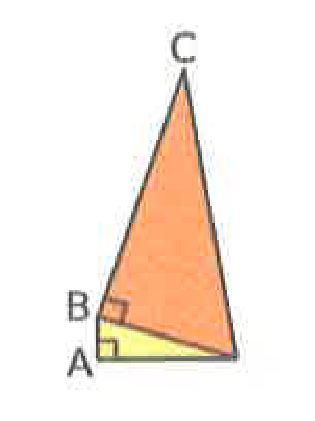
\includegraphics[scale=0.5]{T1}
\end{center}
\end{minipage}
\end{exercice}


\begin{exercice}
Après un violent orage, Julia constate que la foudre a cassé son arbre préféré à 2 m du sol.

La cime touche le sol à 7 m du pied de l’arbre.

\begin{center}
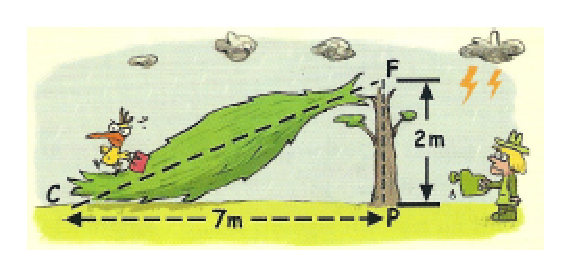
\includegraphics[scale=0.55]{T7}
\end{center}
Quelle était la hauteur de l'arbre avant l'orage, au décimètre près ?

\end{exercice}

\begin{exercice}
\emph{On considère le triangle \emph{BEA} représenté ci-dessous :}

\vspace{0,25cm}

\begin{center}
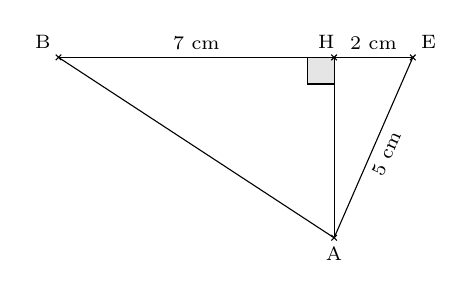
\begin{tikzpicture}[x=0.5cm,y=0.5cm]
\draw[fill=black,fill opacity=0.1] (6.324340988406047,-8.274436458635991E-17) -- (6.324340988406047,-0.6756590115939533) -- (7.0,-0.6756590115939531) -- (7.0,0.0) -- cycle; 
\draw (0.0,-0.0)-- (7.0,0.0);
\draw (7.0,0.0)-- (9.0,0.0);
\draw (9.0,0.0)-- (7.0,-4.58257569495584);
\draw (7.0,-4.58257569495584)-- (7.0,0.0);
\draw (7.0,-4.58257569495584)-- (0.0,-0.0);
\begin{scriptsize}
\draw [color=black] (0.0,-0.0)-- ++(-1.0pt,-1.0pt) -- ++(2.0pt,2.0pt) ++(-2.0pt,0) -- ++(2.0pt,-2.0pt);
\draw[color=black] (-0.4,0.4) node {B};
\draw [color=black] (7.0,0.0)-- ++(-1.0pt,-1.0pt) -- ++(2.0pt,2.0pt) ++(-2.0pt,0) -- ++(2.0pt,-2.0pt);
\draw[color=black] (6.8,0.4) node {H};
\draw [color=black] (9.0,0.0)-- ++(-1.0pt,-1.0pt) -- ++(2.0pt,2.0pt) ++(-2.0pt,0) -- ++(2.0pt,-2.0pt);
\draw[color=black] (9.4,0.4) node {E};
\draw [color=black] (7.0,-4.58257569495584)-- ++(-1.0pt,-1.0pt) -- ++(2.0pt,2.0pt) ++(-2.0pt,0) -- ++(2.0pt,-2.0pt);
\draw[color=black] (7,-5) node {A};
\draw (3.5,0) node[above] {7 cm};
\draw (8,0) node[above] {2 cm};
\draw (8,-2.3) node[below,rotate=66] {5 cm};
\end{scriptsize}
\end{tikzpicture}
\end{center}

\begin{enumerate}
\item Calculer l'aire du triangle BEA, arrondie au mm$^2$. On détaillera les étapes du raisonnement.
\item Calculer la longueur AB. Donner sa valeur exacte et sa valeur arrondie au mm.
\end{enumerate}
\end{exercice}

\begin{exercice}
Un triangle $EFG$ est rectangle en $E$ avec $EG = 7 cm$ et $\widehat{FGE} = 45°$.
\begin{enumerate}
\item Calculer la mesure de l'angle  $\widehat{EFG}$.
\item Calculer, en justifiant, $EF$ et $FG$ (arrondir au mm).
\end{enumerate}
\end{exercice}

\begin{exercice}
Rectangle ou non ?
\begin{enumerate}
\item Le triangle XYZ est tel que  XY =29,8cm ; YZ = 28,1cm et  XZ= 10,2cm.\\
Est-il rectangle ? Justifier.
\item Soit le triangle ALE tel que :	AL = 13,1cm ; LE = 11,2cm ; EA = 6,6 cm.\\
Est-il rectangle ? Justifier.
\end{enumerate}
\end{exercice}

\begin{exercice}
Pour chacun des triangles suivants, déterminer s'il s'agit ou non d'un triangle rectangle et préciser, le cas échéant, quelle est son hypoténuse.

\begin{enumerate}
\item TOP \emph{est un triangle tel que}

OT = 39 cm, OP = 65 cm \emph{et} TP = 52 cm.

\vspace{0.25cm}
\item BUS \emph{est un triangle tel que}

BU = 8 cm, US = 4,5 cm \emph{et} BS = 9,2 cm.
\end{enumerate}
\end{exercice}

\begin{exercice}
On considère le  parallélogramme STOP dessiné à main levée.\\
\begin{minipage}{0.6\linewidth}


Démontrer que le parallélogramme STOP est un rectangle.

\end{minipage}
\hfill
\begin{minipage}{0.3\linewidth}
\begin{center}
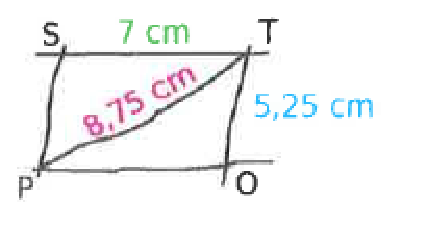
\includegraphics[scale=0.5]{T2}
\end{center}
\end{minipage}
\end{exercice}

\begin{exercice}
Sur la figure ci-contre :

\begin{minipage}{0.6\linewidth}
\begin{itemize}
\item EFGH \emph{est un rectangle} ;
\item EF = 14 m \emph{et} FG = 12 m ;
\item K $\in$ [EH] \emph{et} EK = 4 m ;
\item L $\in$ [EF] \emph{et} EL = 6 m.
\end{itemize}
Le triangle KGL est-il rectangle ?

\end{minipage}
\hfill
\begin{minipage}{0.3\linewidth}
\begin{center}

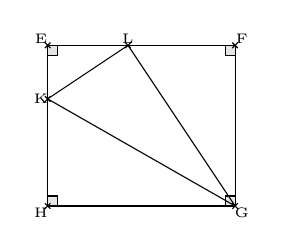
\begin{tikzpicture}[x=0.17cm,y=0.17cm]
\draw[fill=black,fill opacity=0.1] (0.7415589313755807,0.0) -- (0.7415589313755808,0.7415589313755807) -- (4.540738858441183E-17,0.7415589313755807) -- (0.0,-0.0) -- cycle; 
\draw[fill=black,fill opacity=0.1] (13.25844106862442,12.0) -- (13.25844106862442,11.25844106862442) -- (14.0,11.25844106862442) -- (14.0,12.0) -- cycle; 
\draw[fill=black,fill opacity=0.1] (4.540738858441183E-17,11.25844106862442) -- (0.7415589313755808,11.25844106862442) -- (0.7415589313755807,12.0) -- (0.0,12.0) -- cycle; 
\draw[fill=black,fill opacity=0.1] (14.0,0.7415589313755807) -- (13.25844106862442,0.7415589313755808) -- (13.25844106862442,9.081477716882366E-17) -- (14.0,0.0) -- cycle; 
\draw (0.0,-0.0)-- (0.0,12.0);
\draw (0.0,12.0)-- (14.0,12.0);
\draw (14.0,12.0)-- (14.0,0.0);
\draw (14.0,0.0)-- (0.0,-0.0);
\draw (0.0,8.0)-- (6.0,12.0);
\draw (6.0,12.0)-- (14.0,0.0);
\draw (14.0,0.0)-- (0.0,8.0);
\begin{tiny}
\draw [color=black] (0.0,-0.0)-- ++(-1.0pt,-1.0pt) -- ++(2.0pt,2.0pt) ++(-2.0pt,0) -- ++(2.0pt,-2.0pt);
\draw[color=black] (-0.5,-0.5) node {H};
\draw [color=black] (14.0,0.0)-- ++(-1.0pt,-1.0pt) -- ++(2.0pt,2.0pt) ++(-2.0pt,0) -- ++(2.0pt,-2.0pt);
\draw[color=black] (14.5,-0.5) node {G};
\draw [color=black] (0.0,12.0)-- ++(-1.0pt,-1.0pt) -- ++(2.0pt,2.0pt) ++(-2.0pt,0) -- ++(2.0pt,-2.0pt);
\draw[color=black] (-0.5,12.5) node {E};
\draw [color=black] (14.0,12.0)-- ++(-1.0pt,-1.0pt) -- ++(2.0pt,2.0pt) ++(-2.0pt,0) -- ++(2.0pt,-2.0pt);
\draw[color=black] (14.5,12.5) node {F};
\draw [color=black] (0.0,8.0)-- ++(-1.0pt,-1.0pt) -- ++(2.0pt,2.0pt) ++(-2.0pt,0) -- ++(2.0pt,-2.0pt);
\draw[color=black] (-0.5,8) node {K};
\draw [color=black] (6.0,12.0)-- ++(-1.0pt,-1.0pt) -- ++(2.0pt,2.0pt) ++(-2.0pt,0) -- ++(2.0pt,-2.0pt);
\draw[color=black] (6,12.5) node {L};
\end{tiny}
\end{tikzpicture}
\end{center}
\end{minipage}
\end{exercice}

\newpage

\serie{Théorème de Thalès}

\begin{exercice}
Sur la figure ci-dessous, les droites (LN) et (RO) sont paralléles (les longueurs sont en centimètres).

Les droites (RN) et (OA) sont sécantes en L.

Calculer les longueurs LR et AO.


\begin{center}
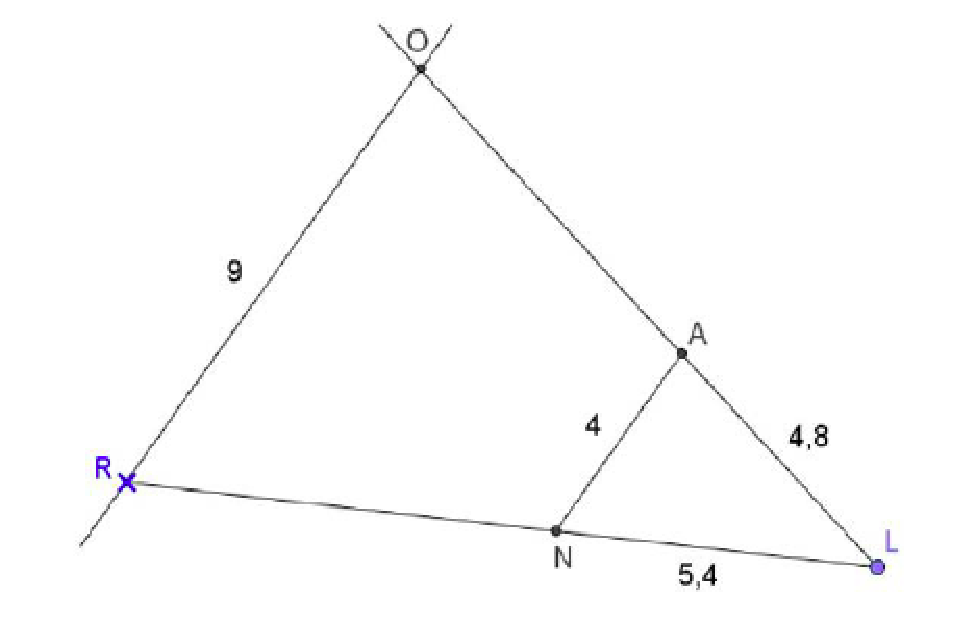
\includegraphics[scale=0.4]{T8}
\end{center}
\end{exercice}

\begin{exercice}
On suppose que $(AB)\parallel (CD)$, $AB = 72$, $CD = 96$, $SC = 84$ et $SD = 72$. Les mesures sont en millimètres.

\begin{center}
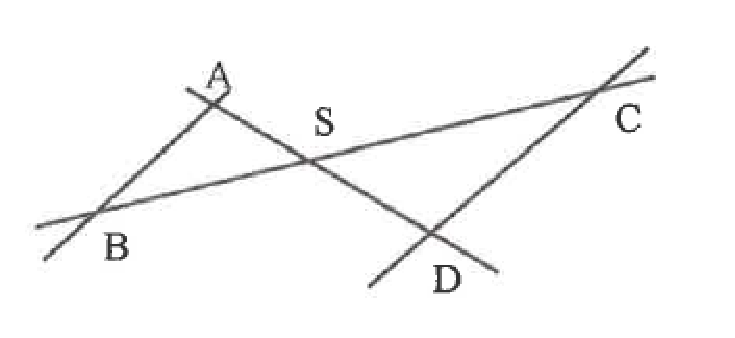
\includegraphics[scale=0.5]{T3}
\end{center}

Trouver $SA$ et $SB$.
\end{exercice}

\begin{exercice}
Lors de son premier voyage en Egypte, Thalès applique le théorème qui porte aujourd'hui son nom pour mesurer la hauteur de la grande pyramide de Kheops.

\begin{center}
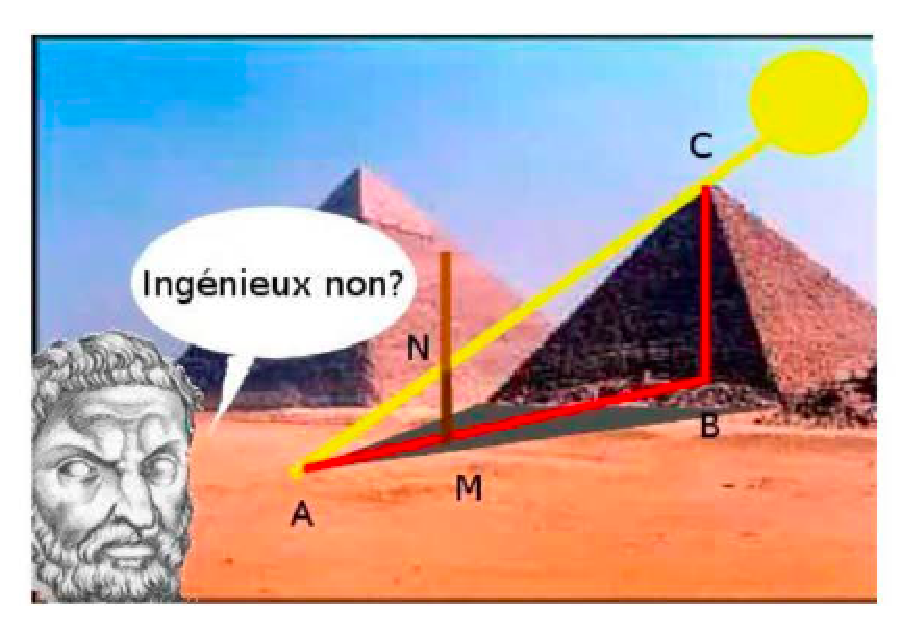
\includegraphics[scale=0.4]{T9}
\end{center}

Les points A, M, B sont alignés, les points A, N, C aussi.

Les droites (MN) et (BC) sont parallèles. On donne:

AM = 5,4 m; MN = 1,39 m et MB = 534,6 m.

Calculer la hauteur BC de la pyramide de Kheops.

Citation de Thalès: "Le rapport que j'entretiens avec mon ombre est le même que celui de la pyramide avec la sienne."
\end{exercice}

\begin{exercice}
On a : OM= 2,8 cm ; ON = 5,4 cm ; OS= 2,7 cm
et OT = 1,4 cm.

\begin{center}
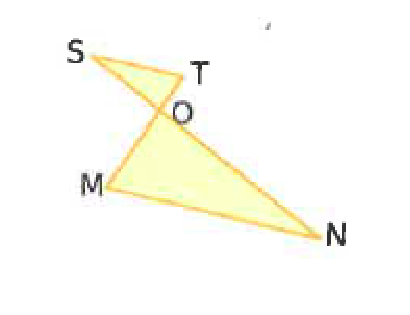
\includegraphics[scale=0.5]{T4}
\end{center}
Démontrer que les droites MN et ST sont parallèles.
\end{exercice}

\begin{exercice}
L'unité de longueur choisie est le mètre. 
\begin{center}
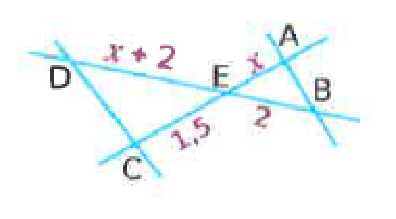
\includegraphics[scale=0.5]{T5}
\end{center}

\begin{enumerate}
\item Pour $x = 2,5$, les droites (AB) et (CD) ne sont pas parallèles. 
Vrai ou faux? Expliquer la démarche.
\item Pour $x = 1$, les droites (AB) et (DC) ne sont pas parallèles. Vrai ou faux ? Expliquer la démarche.
\end{enumerate}
\end{exercice}

\begin{exercice}
ABC est un triangle. D est un point de [AB] et E est un point de (AC) n'appartenant pas à [AC]. On donne AB = 4cm ; AC = 3cm ; AD = 1,2cm et AE = 0,9cm.\\
Alixien a écrit sur sa copie :\\
« Les droites EC et DB sont sécantes en A.\\\\
 D'une part, $\dfrac{AD}{AB}=\dfrac{1,2}{4}=\dfrac{12}{40}=\dfrac{3}{10}$.\\\\
D'autre part, $\dfrac{AE}{AC}=\dfrac{0,9}{3}=\dfrac{9}{30}=\dfrac{3}{10}$.\\\\
Comme $\dfrac{AD}{AB}=\dfrac{AE}{AC}$ alors les droites BC et ED sont parallèles. » 

\begin{enumerate}
\item Quel théorème Alixien a-t-il utilisé ?
\item La réponse d'Alixien est-elle juste ? Sinon, rédiger la bonne réponse..
\end{enumerate}
\end{exercice}

\newpage

%%%%%%%%%%%%%%%%%%%%%%%%%%%%%%%%%%%%%%%%%%%%%%%%%%%

\serie{Divers}

\begin{exercice}
Sur la figure, les droites (EF) et (MP) sont parallèles.
\begin{center}
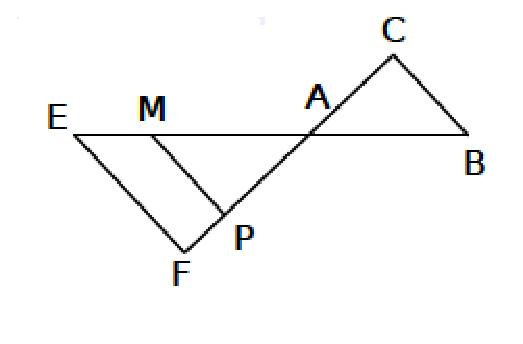
\includegraphics[scale=0.5]{T10}
\end{center}

On sait que AM=6 cm ; MP=4,8cm ; AP=3,6 cm ; EF=6 cm ; AC=4,5 cm et AB=7,5 cm .

\begin{enumerate}
\item Démontrer que le triangle AMP est un triangle rectangle.
\item Calculer AE puis la longueur ME.
\item Démontrer que les droites (MP) et (BC) sont parallèles.
\end{enumerate}
\end{exercice}


\begin{exercice}
Pour consolider un bâtiment, des charpentiers  ont construit un contrefort en bois (les mesures sont en mètre).

\begin{minipage}{0.5\linewidth}
\begin{enumerate}
\item En considérant que le montant [BS] est perpendiculaire au sol, calculer la longueur AS.
\item Calculer les longueurs SM et SN.
\item Démontrer que la traverse [MN] est bien parallèle au sol.
\end{enumerate}

\end{minipage}
\hfill
\begin{minipage}{0.4\linewidth}
\begin{center}
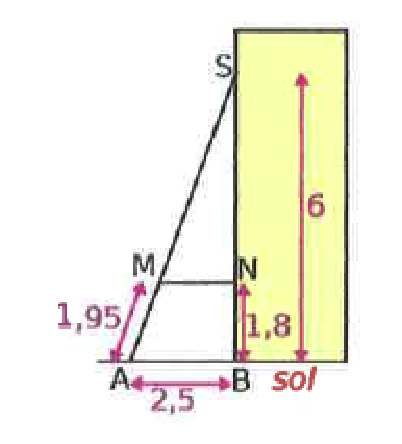
\includegraphics[scale=0.5]{T6}
\end{center}
\end{minipage}
\end{exercice} 










